\documentclass[11pt]{article}
\usepackage[margin=0.75in]{geometry}
\usepackage{graphicx}
\usepackage{booktabs}
\usepackage{float}
\usepackage{hyperref}
\usepackage{amsmath}
\usepackage{longtable}
\usepackage{array}

\title{Computational Prediction of Drug-Induced Heart Damage:\\
ADMET-AI vs SwissADME Comparison\\
\large Analysis of 25 Cardiac RODEO Drugs}
\author{Cardiac RODEO Project}
\date{\today}

\begin{document}
\maketitle

\begin{abstract}
This report compares two computational approaches for predicting drug-induced heart damage:
ADMET-AI (41 ADMET properties) and SwissADME (43 physicochemical properties).
We replicate published DICTrank benchmark results, evaluate predictions on 25 Cardiac RODEO drugs,
and train new models using Leave-One-Out Cross-Validation (LOOCV) and scaffold-balanced CV.
\end{abstract}

\section{DICTrank Training Results}

We trained XGBoost models on the DICTrank dataset (555 drugs: 293 most DICT concern, 262 no concern)
using 10-fold scaffold-balanced cross-validation.

\begin{table}[H]
\centering
\caption{DICTrank Training Results (10-Fold CV)}
\begin{tabular}{lccc}
\toprule
\textbf{Model} & \textbf{ROC AUC} & \textbf{PR AUC} & \textbf{Accuracy} \\
\midrule
ADMET-AI & 0.72 & 0.75 & 0.64 \\
SwissADME & 0.66 & 0.68 & 0.60 \\
\bottomrule
\end{tabular}
\end{table}

\begin{figure}[H]
\centering
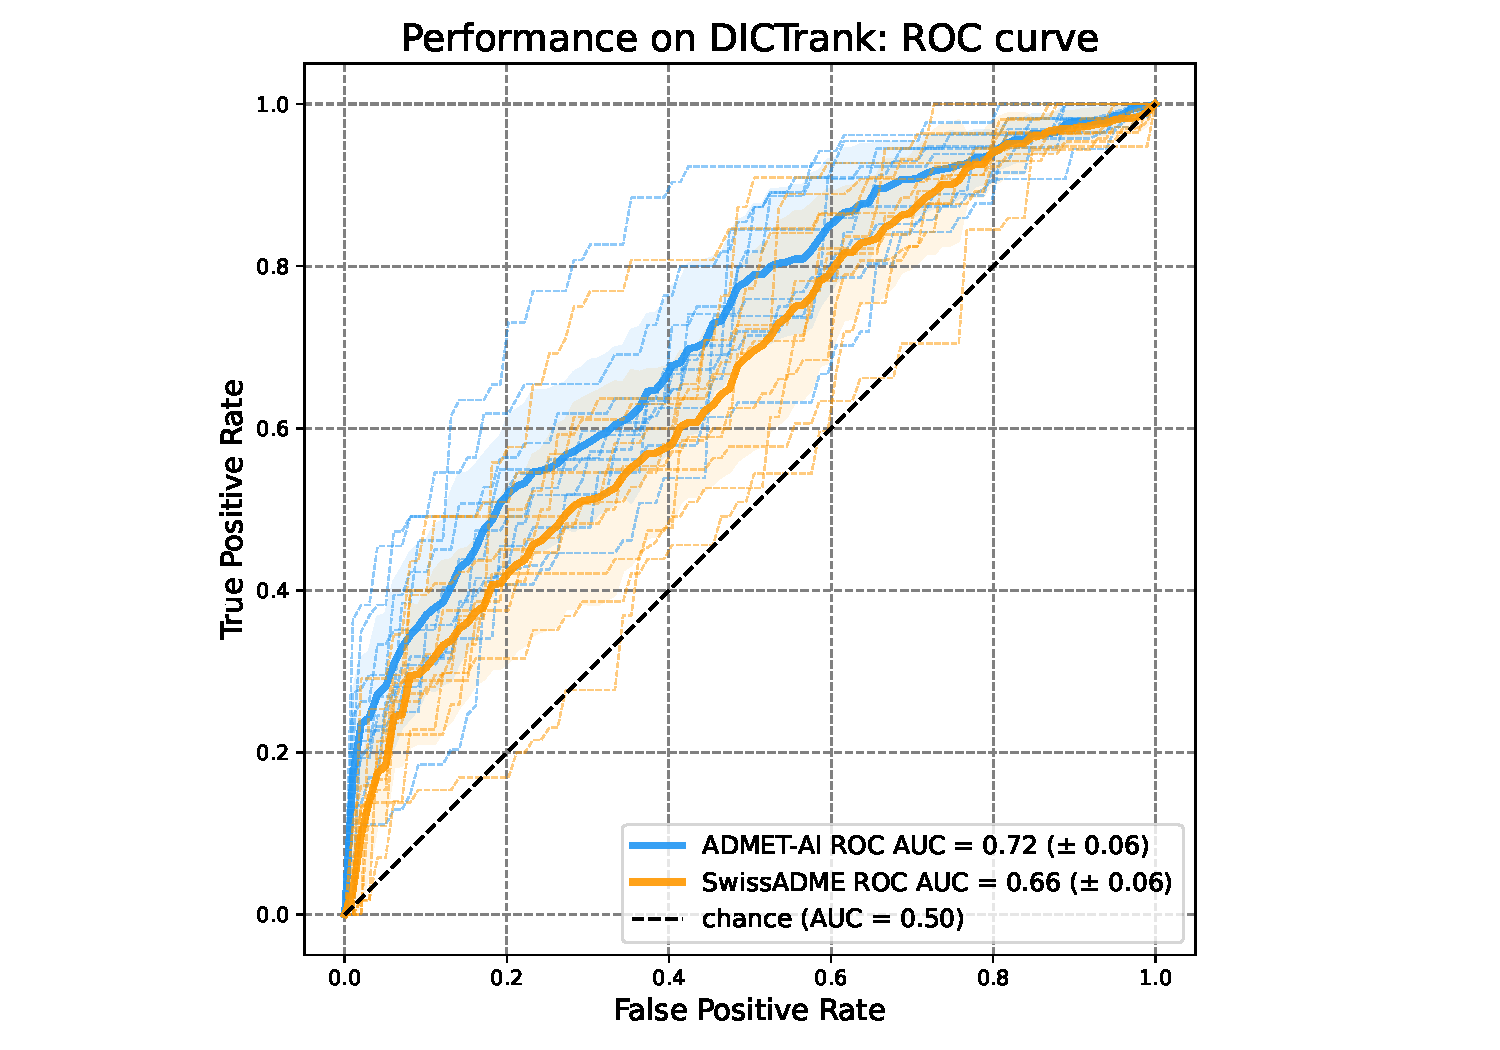
\includegraphics[width=0.7\textwidth]{figures/dictrank_retrain_roc.pdf}
\caption{ROC curves from DICTrank training (10-fold scaffold-balanced cross-validation on 555 drugs).}
\end{figure}

\begin{figure}[H]
\centering
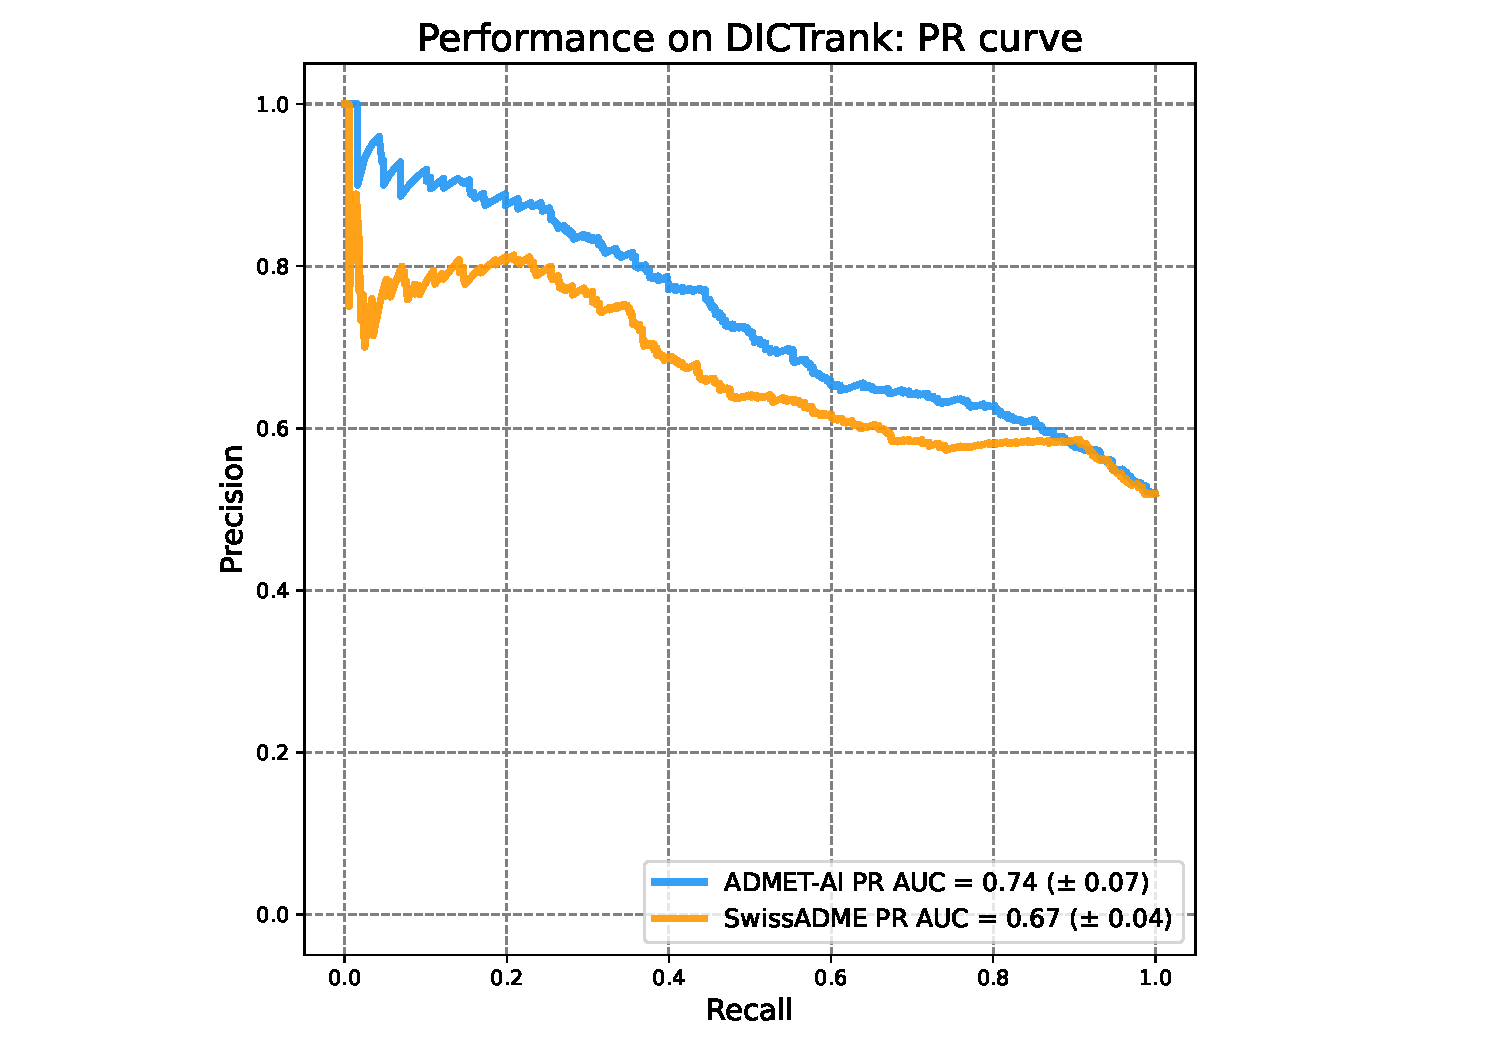
\includegraphics[width=0.7\textwidth]{figures/dictrank_retrain_pr.pdf}
\caption{Precision-recall curves from DICTrank training (10-fold scaffold-balanced cross-validation on 555 drugs).}
\end{figure}

\section{Cardiac RODEO Drug Dataset}

Our dataset contains 25 drugs with experimentally determined cardiac outcomes:
\begin{itemize}
    \item Heart Damage Positive: 20/25 drugs (80\%)
    \item Heart Damage Negative: 5/25 drugs (20\%)
\end{itemize}

\begin{longtable}{lcc>{\raggedright\arraybackslash}p{7cm}}
\caption{Drug Database with SMILES and Sources} \\
\toprule
\textbf{Drug} & \textbf{CID} & \textbf{MW} & \textbf{SMILES} \\
\midrule
\endfirsthead
\toprule
\textbf{Drug} & \textbf{CID} & \textbf{MW} & \textbf{SMILES} \\
\midrule
\endhead
    Amiodarone & 2157 & 645.3 & \begin{tabular}[t]{@{}l@{}}\texttt{CCCCC1=C(C2=CC=CC=C2O1)C(=O)C3=CC(=}\\\texttt{C(C(=C3)I)OCCN(CC)CC)I}\end{tabular} \\
    Bortezomib & 387447 & 384.2 & \begin{tabular}[t]{@{}l@{}}\texttt{B(C(CC(C)C)NC(=O)C(CC1=CC=CC=C1)NC(}\\\texttt{=O)C2=NC=CN=C2)(O)O}\end{tabular} \\
    Chlorpromazine & 2726 & 318.9 & \begin{tabular}[t]{@{}l@{}}\texttt{CN(C)CCCN1C2=CC=CC=C2SC3=C1C=C(C=C3}\\\texttt{)Cl}\end{tabular} \\
    Cobimetinib & 16222096 & 531.3 & \begin{tabular}[t]{@{}l@{}}\texttt{C1CCNC(C1)C2(CN(C2)C(=O)C3=C(C(=C(C}\\\texttt{=C3)F)F)NC4=C(C=C(C=C4)I)F)O}\end{tabular} \\
    Dactinomycin & 457193 & 1255.4 & \begin{tabular}[t]{@{}l@{}}\texttt{CC1C(C(=O)NC(C(=O)N2CCCC2C(=O)N(CC(}\\\texttt{=O)N(C(C(=O)O1)C(C)C)C)C)C(C)C)NC(=}\\\texttt{O)C3=C4C(=C(C=C3)C)OC5=C(C(=O)C(=C(}\\\texttt{C5=N4)C(=O)NC6C(OC(=O)C(N(C(=O)CN(C}\\\texttt{(=O)C7CCCN7C(=O)C(NC6=O)C(C)C)C)C)C}\\\texttt{(C)C)C)N)C}\end{tabular} \\
    Daunorubicin & 30323 & 527.5 & \begin{tabular}[t]{@{}l@{}}\texttt{CC1C(C(CC(O1)OC2CC(CC3=C2C(=C4C(=C3}\\\texttt{O)C(=O)C5=C(C4=O)C(=CC=C5)OC)O)(C(=}\\\texttt{O)C)O)N)O}\end{tabular} \\
    Doxorubicin & 31703 & 543.5 & \begin{tabular}[t]{@{}l@{}}\texttt{CC1C(C(CC(O1)OC2CC(CC3=C2C(=C4C(=C3}\\\texttt{O)C(=O)C5=C(C4=O)C(=CC=C5)OC)O)(C(=}\\\texttt{O)CO)O)N)O}\end{tabular} \\
    Epirubicin & 41867 & 543.5 & \begin{tabular}[t]{@{}l@{}}\texttt{CC1C(C(CC(O1)OC2CC(CC3=C2C(=C4C(=C3}\\\texttt{O)C(=O)C5=C(C4=O)C(=CC=C5)OC)O)(C(=}\\\texttt{O)CO)O)N)O}\end{tabular} \\
    Erlotinib & 176870 & 393.4 & \begin{tabular}[t]{@{}l@{}}\texttt{COCCOC1=C(C=C2C(=C1)C(=NC=N2)NC3=CC}\\\texttt{=CC(=C3)C#C)OCCOC}\end{tabular} \\
    Etomoxir & 9840324 & 326.8 & \begin{tabular}[t]{@{}l@{}}\texttt{CCOC(=O)C1(CO1)CCCCCCOC2=CC=C(C=C2)}\\\texttt{Cl}\end{tabular} \\
    Gemcitibine & 60750 & 263.2 & \begin{tabular}[t]{@{}l@{}}\texttt{C1=CN(C(=O)N=C1N)C2C(C(C(O2)CO)O)(F}\\\texttt{)F}\end{tabular} \\
    Ibrutinib & 24821094 & 440.5 & \begin{tabular}[t]{@{}l@{}}\texttt{C=CC(=O)N1CCCC(C1)N2C3=NC=NC(=C3C(=}\\\texttt{N2)C4=CC=C(C=C4)OC5=CC=CC=C5)N}\end{tabular} \\
    Ibuprofen & 3672 & 206.3 & \begin{tabular}[t]{@{}l@{}}\texttt{CC(C)CC1=CC=C(C=C1)C(C)C(=O)O}\end{tabular} \\
    Isoproterenol & 3779 & 211.3 & \begin{tabular}[t]{@{}l@{}}\texttt{CC(C)NCC(C1=CC(=C(C=C1)O)O)O}\end{tabular} \\
    Mexiletine & 4178 & 179.3 & \begin{tabular}[t]{@{}l@{}}\texttt{CC1=C(C(=CC=C1)C)OCC(C)N}\end{tabular} \\
    Nifedipine & 4485 & 346.3 & \begin{tabular}[t]{@{}l@{}}\texttt{CC1=C(C(C(=C(N1)C)C(=O)OC)C2=CC=CC=}\\\texttt{C2[N+](=O)[O-])C(=O)OC}\end{tabular} \\
    Panobinostat & 6918837 & 349.4 & \begin{tabular}[t]{@{}l@{}}\texttt{CC1=C(C2=CC=CC=C2N1)CCNCC3=CC=C(C=C}\\\texttt{3)C=CC(=O)NO}\end{tabular} \\
    Plicamycin & 163659 & 1085.1 & \begin{tabular}[t]{@{}l@{}}\texttt{CC1C(C(CC(O1)OC2CC(OC(C2O)C)OC3=CC4}\\\texttt{=CC5=C(C(=O)C(C(C5)C(C(=O)C(C(C)O)O}\\\texttt{)OC)OC6CC(C(C(O6)C)O)OC7CC(C(C(O7)C}\\\texttt{)O)OC8CC(C(C(O8)C)O)(C)O)C(=C4C(=C3}\\\texttt{C)O)O)O)O}\end{tabular} \\
    Rosiglitazone & 77999 & 357.4 & \begin{tabular}[t]{@{}l@{}}\texttt{CN(CCOC1=CC=C(C=C1)CC2C(=O)NC(=O)S2}\\\texttt{)C3=CC=CC=N3}\end{tabular} \\
    Sotalol & 5253 & 272.4 & \begin{tabular}[t]{@{}l@{}}\texttt{CC(C)NCC(C1=CC=C(C=C1)NS(=O)(=O)C)O}\end{tabular} \\
    Sunitinib & 5329102 & 398.5 & \begin{tabular}[t]{@{}l@{}}\texttt{CCN(CC)CCNC(=O)C1=C(NC(=C1C)C=C2C3=}\\\texttt{C(C=CC(=C3)F)NC2=O)C}\end{tabular} \\
    Vandetanib & 3081361 & 475.4 & \begin{tabular}[t]{@{}l@{}}\texttt{CN1CCC(CC1)COC2=C(C=C3C(=C2)N=CN=C3}\\\texttt{NC4=C(C=C(C=C4)Br)F)OC}\end{tabular} \\
    Vincristine & 5978 & 825.0 & \begin{tabular}[t]{@{}l@{}}\texttt{CCC1(CC2CC(C3=C(CCN(C2)C1)C4=CC=CC=}\\\texttt{C4N3)(C5=C(C=C6C(=C5)C78CCN9C7C(C=C}\\\texttt{C9)(C(C(C8N6C=O)(C(=O)OC)O)OC(=O)C)}\\\texttt{CC)OC)C(=O)OC)O}\end{tabular} \\
    Vioxx & 5090 & 314.4 & \begin{tabular}[t]{@{}l@{}}\texttt{CS(=O)(=O)C1=CC=C(C=C1)C2=C(C(=O)OC}\\\texttt{2)C3=CC=CC=C3}\end{tabular} \\
    Vorinostat & 5311 & 264.3 & \begin{tabular}[t]{@{}l@{}}\texttt{C1=CC=C(C=C1)NC(=O)CCCCCCC(=O)NO}\end{tabular} \\
\bottomrule
\end{longtable}

All drugs sourced from PubChem (https://pubchem.ncbi.nlm.nih.gov).

\section{DICTrank Model Predictions on 25 Drugs}

DICTrank-trained models were applied to predict heart damage for the 25 Cardiac RODEO drugs.

\begin{table}[H]
\centering
\caption{DICTrank Model Performance on 25 Cardiac RODEO Drugs}
\begin{tabular}{lcccccc}
\toprule
\textbf{Model} & \textbf{Accuracy} & \textbf{ROC AUC} & \textbf{TP} & \textbf{FN} & \textbf{TN} & \textbf{FP} \\
\midrule
ADMET-AI & 0.60 & 0.50 & 13 & 7 & 2 & 3 \\
SwissADME & 0.48 & 0.47 & 10 & 10 & 2 & 3 \\
\bottomrule
\end{tabular}
\end{table}

\begin{figure}[H]
\centering

\includegraphics[width=\textwidth]{figures/dictrank_predictions.pdf}
\caption{DICTrank model predictions for each drug. Circles = ADMET-AI, Squares = SwissADME.}
\end{figure}

\begin{longtable}{lccccc}
\caption{Individual Drug Predictions (DICTrank Models)} \\
\toprule
\textbf{Drug} & \textbf{True HD} & \textbf{ADMET Prob} & \textbf{Pred} & \textbf{Swiss Prob} & \textbf{Pred} \\
\midrule
\endfirsthead
\toprule
\textbf{Drug} & \textbf{True HD} & \textbf{ADMET Prob} & \textbf{Pred} & \textbf{Swiss Prob} & \textbf{Pred} \\
\midrule
\endhead
    Amiodarone & Yes & 0.000 & Low & 1.000 & High \\
    Bortezomib & Yes & 1.000 & High & 1.000 & High \\
    Chlorpromazine & Yes & 1.000 & High & 0.000 & Low \\
    Cobimetinib & Yes & 1.000 & High & 1.000 & High \\
    Dactinomycin & No & 1.000 & High & 0.055 & Low \\
    Daunorubicin & Yes & 1.000 & High & 1.000 & High \\
    Doxorubicin & Yes & 1.000 & High & 1.000 & High \\
    Epirubicin & Yes & 1.000 & High & 1.000 & High \\
    Erlotinib & No & 0.000 & Low & 0.000 & Low \\
    Etomoxir & No & 0.000 & Low & 1.000 & High \\
    Gemcitibine & Yes & 1.000 & High & 0.049 & Low \\
    Ibrutinib & Yes & 1.000 & High & 0.000 & Low \\
    Ibuprofen & Yes & 1.000 & High & 0.000 & Low \\
    Isoproterenol & Yes & 1.000 & High & 1.000 & High \\
    Mexiletine & No & 1.000 & High & 1.000 & High \\
    Nifedipine & Yes & 1.000 & High & 1.000 & High \\
    Panobinostat & Yes & 0.447 & Low & 0.000 & Low \\
    Plicamycin & No & 1.000 & High & 1.000 & High \\
    Rosiglitazone & Yes & 0.000 & Low & 0.000 & Low \\
    Sotalol & Yes & 1.000 & High & 0.000 & Low \\
    Sunitinib & Yes & 1.000 & High & 1.000 & High \\
    Vandetanib & Yes & 0.000 & Low & 0.000 & Low \\
    Vincristine & Yes & 0.000 & Low & 1.000 & High \\
    Vioxx & Yes & 0.000 & Low & 0.000 & Low \\
    Vorinostat & Yes & 0.000 & Low & 0.000 & Low \\
\bottomrule
\end{longtable}

\section{LOOCV Models (Trained on 25 Drugs)}

\subsection{Performance Metrics}

\begin{table}[H]
\centering
\caption{LOOCV Model Performance}
\begin{tabular}{lcccccc}
\toprule
\textbf{Model} & \textbf{Accuracy} & \textbf{ROC AUC} & \textbf{TP} & \textbf{FN} & \textbf{TN} & \textbf{FP} \\
\midrule
ADMET-AI & 0.52 & 0.48 & 13 & 7 & 0 & 5 \\
SwissADME & 0.68 & 0.48 & 17 & 3 & 0 & 5 \\
\bottomrule
\end{tabular}
\end{table}

\begin{figure}[H]
\centering

\includegraphics[width=0.8\textwidth]{figures/accuracy_comparison.pdf}
\caption{Accuracy comparison between DICTrank, Scaffold CV, and LOOCV models.}
\end{figure}

\subsection{ROC Curves}

\begin{figure}[H]
\centering

\includegraphics[width=0.75\textwidth]{figures/loocv_roc.pdf}
\caption{ROC curves for LOOCV models trained on 25 Cardiac RODEO drugs.}
\end{figure}

\subsection{Confusion Matrices}

\begin{figure}[H]
\centering

\includegraphics[width=\textwidth]{figures/loocv_confusion_matrices.pdf}
\caption{Confusion matrices for LOOCV models showing classification performance.}
\end{figure}

\subsection{Drug-by-Drug Predictions}

\begin{figure}[H]
\centering

\includegraphics[width=\textwidth]{figures/loocv_predictions.pdf}
\caption{LOOCV model predictions for each drug. Circles = ADMET-AI, Squares = SwissADME.}
\end{figure}

\section{Scaffold-Balanced CV Models (25 Drugs)}

\begin{table}[H]
\centering
\caption{Scaffold-Balanced CV Model Performance (25 Drugs)}
\begin{tabular}{lcccccc}
\toprule
\textbf{Model} & \textbf{Accuracy} & \textbf{ROC AUC (mean)} & \textbf{TP} & \textbf{FN} & \textbf{TN} & \textbf{FP} \\
\midrule
ADMET-AI & 0.68 & 0.53 & 10 & 10 & 2 & 3 \\
SwissADME & 0.60 & 0.57 & 9 & 11 & 2 & 3 \\
\bottomrule
\end{tabular}
\end{table}

\begin{figure}[H]
\centering

\includegraphics[width=\textwidth]{figures/scaffold_predictions.pdf}
\caption{Scaffold-balanced CV predictions for each drug. Circles = ADMET-AI, Squares = SwissADME.}
\end{figure}

\section{Overall Comparison}

\begin{figure}[H]
\centering

\includegraphics[width=0.85\textwidth]{figures/auc_comparison.pdf}
\caption{AUC comparison across all settings: DICTrank training (10-fold CV), DICTrank applied to 25 drugs, scaffold CV on 25 drugs, and LOOCV on 25 drugs.}
\end{figure}

\section{Discussion}

\begin{enumerate}
    \item \textbf{DICTrank Replication}: Our training on DICTrank achieved ROC AUC of 0.72 (ADMET-AI) and 0.66 (SwissADME), consistent with published results.

    \item \textbf{Domain Shift}: When applied to Cardiac RODEO drugs, performance differs (ADMET-AI: 0.50, SwissADME: 0.47), indicating differences between clinical DICT labels and organoid-measured heart damage.

    \item \textbf{Scaffold CV on 25 Drugs}: Scaffold-balanced CV yields mean ROC AUC of 0.53 (ADMET-AI) and 0.57 (SwissADME), reflecting generalization across scaffolds within the small panel.

    \item \textbf{LOOCV Performance}: Models trained on 25 drugs achieved ADMET-AI AUC = 0.48 and SwissADME AUC = 0.48. Small sample size limits generalization.

    \item \textbf{Class Imbalance}: With 20/25 positive cases (80\%), the dataset is imbalanced.
\end{enumerate}

\section{Conclusion}

Both ADMET-AI and SwissADME provide predictive signal for drug-induced heart damage. Our DICTrank training replicates published results. Performance variation on Cardiac RODEO data suggests organoid-measured cardiac effects may differ from clinical DICT labels.

\section*{References}

Mukherjee P, et al. (2025). ADMET-AI Enables Interpretable Predictions of Drug-Induced Cardiotoxicity. \textit{Clinical Pharmacology \& Therapeutics}.

\end{document}
